\chapter{Tecnologias e Ferramentas Utilizadas}
% OU \chapter{Trabalhos Relacionados}
% OU \chapter{Engenharia de Software}
% OU \chapter{Tecnologias e Ferramentas Utilizadas}
\label{chap:tecno-ferra}

\section{Introdução}
\label{chap3:sec:intro}
O capítulo 3 é dedicado à identificação das ferramentas e tecnologias usadas para desenvolver este projeto. Foram usadas algumas das seguintes ferramentas: \emph{JavaFx} para desenvolver a interface gráfica da aplicação, a biblioteca \emph{JSOUP} uma ferramenta que permite analisar um documento \emph{HTML} e \emph{GitHub} para controlo de versões.

\section{Recursos Utilizados}
\label{chap3:sec:...}

\subsection{NetBeans}
O \emph{NetBBeans} é um ambiente de desenvolvimento de código, onde é possível desenvolver uma grande variedade de linguagens, dentro das quais \emph{Java}, usada neste projeto.
Auxilia programadores a escrever, compilar, no \emph{debug} de código e até mesmo a instalar aplicações. \par
A sua estrutura está feita de forma a simplificar o desenvolvimento e aumentar a produtividade, uma vez que reúne numa única aplicação todas as funcionalidades descritas anteriormente.\par
O \emph{NetBeans} fornece uma base sólida para a criação de projetos, possui um grande conjunto de bibliotecas e \ac{API}, além de uma documentação vasta. Isto faz com que o utilizador escreva o seu código de uma forma mais rápida. \par
Optei por escolher o \emph{NetBeans} porque já tinha experiência anterior na sua utilização e pareceu a mais adequada para usar em conjunto com o \emph{SceneBuiler}.

\subsection{SceneBuilder}
O \emph{SceneBuilder} é uma plataforma de desenvolvimento de ambientes gráficos, que permite criar rapidamente uma aplicação \emph{JavaFx}, sem recurso a código.\par 
Os utilizadores podem arrastar componentes, modificar as suas propriedades, aplicar estilos e o código \emph{FXML} é gerado automaticamente. Esse ficheiro \emph{FXML} é combinado com código \emph{Java}.\par
Permite moldar facilmente o ambiente gráfico da aplicação e adequa-lo às nossas necessidades. O código \emph{FXML} é gerado automaticamente, separadamente da interface lógica da programação. É possível abrir o ficheiro \emph{FXML} e editar o seu código.\par
A qualquer momento da criação do projeto, é possível pré-visualizar a aplicação durante o seu desenvolvimento.

\vspace{0,07cm}
\begin{figure}[H]
\centering
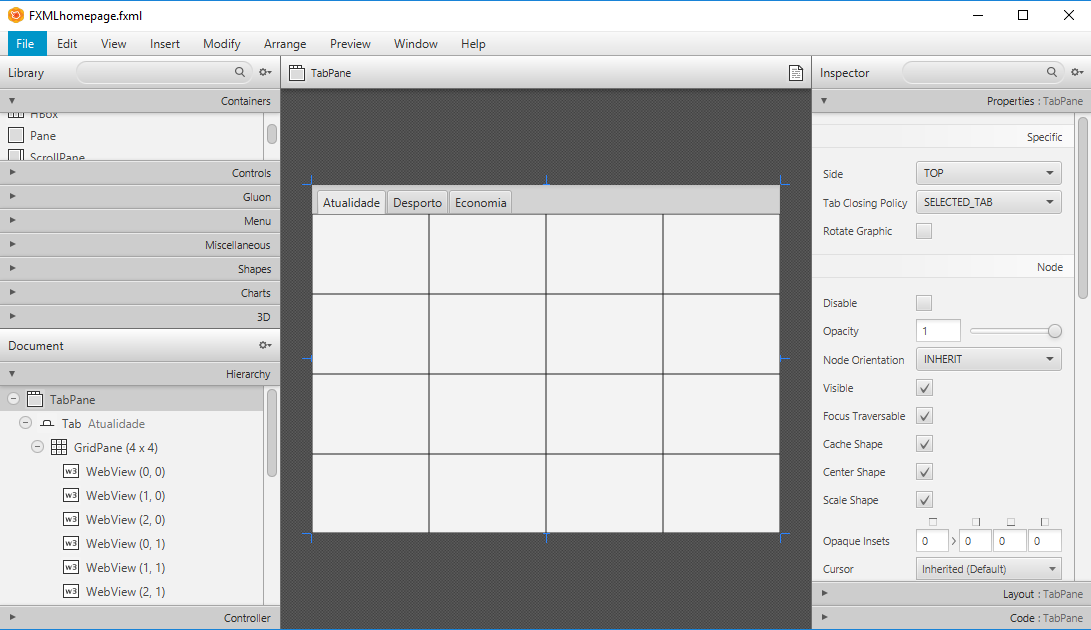
\includegraphics[scale=0.4]{imagens/scene_builder.PNG}
\caption{\emph{Scene Builder}.}
\label{fig:scenebuilder}
\end{figure}
Na figura \ref{fig:scenebuilder} é possível ver uma interface que foi desenvolvida no projeto, permitiu criar de forma rápida uma página que contem muitos elementos.
Foi usado para desenvolver o ambiente gráfico do projeto, fazendo uma ligação rápida com o código \emph{Java}.

\subsection{JavaFx}
\emph{JavaFX} é uma plataforma que permite desenvolver aplicações com interface gráfica com base na programação por eventos. Os \emph{eventos} tratam-se nada mais do que a captura de ações desencadeadas pelo utilizador, tais como, carregar num botão ou numa imagem. Quando isso acontece certos eventos são desencadeados, originando uma resposta. \par
O \emph{JavaFx} interage com o utilizador de acordo com o modelo \ac{MVC}, este consiste em dividir uma aplicação em três partes interligadas. Este modelo é usado para separar as representações internas da informação da forma como a informação é apresentada e aceite pelo utilizador.

\vspace{0,07cm}
\begin{figure}[H]
\centering
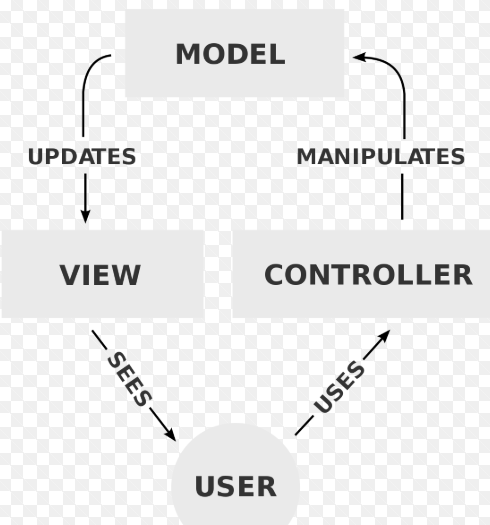
\includegraphics[scale=0.5]{imagens/mvc.PNG}
\caption{Diagrama de interacções do \ac{MVC}.}
\label{fig:gestao}
\end{figure}

Na figura 3.2 está representado o diagrama de interações do modelo \ac{MVC}. Observamos que o \emph{Model} é a componente central, é independente do utilizador e gere os dados, a lógica e regras da aplicação.
A \emph{View} pode ser qualquer representação da informação, tais como um gráfico ou um diagrama. 
A terceira parte \emph{Controller} aceita o \emph{input} e converte-o em comandos para serem interpretados pelo \emph{Model}


Em conjunto com o \emph{SceneBuilder}, o \emph{JavaFx} demonstrou ser uma excelente ferramenta para o desenvolvimento de aplicações com interface gráfica, em conjunto estas duas ferramentas foram usadas para desenvolver a seguinte interface gráfica: 

\vspace{0,07cm}
\begin{figure}[H]
\centering
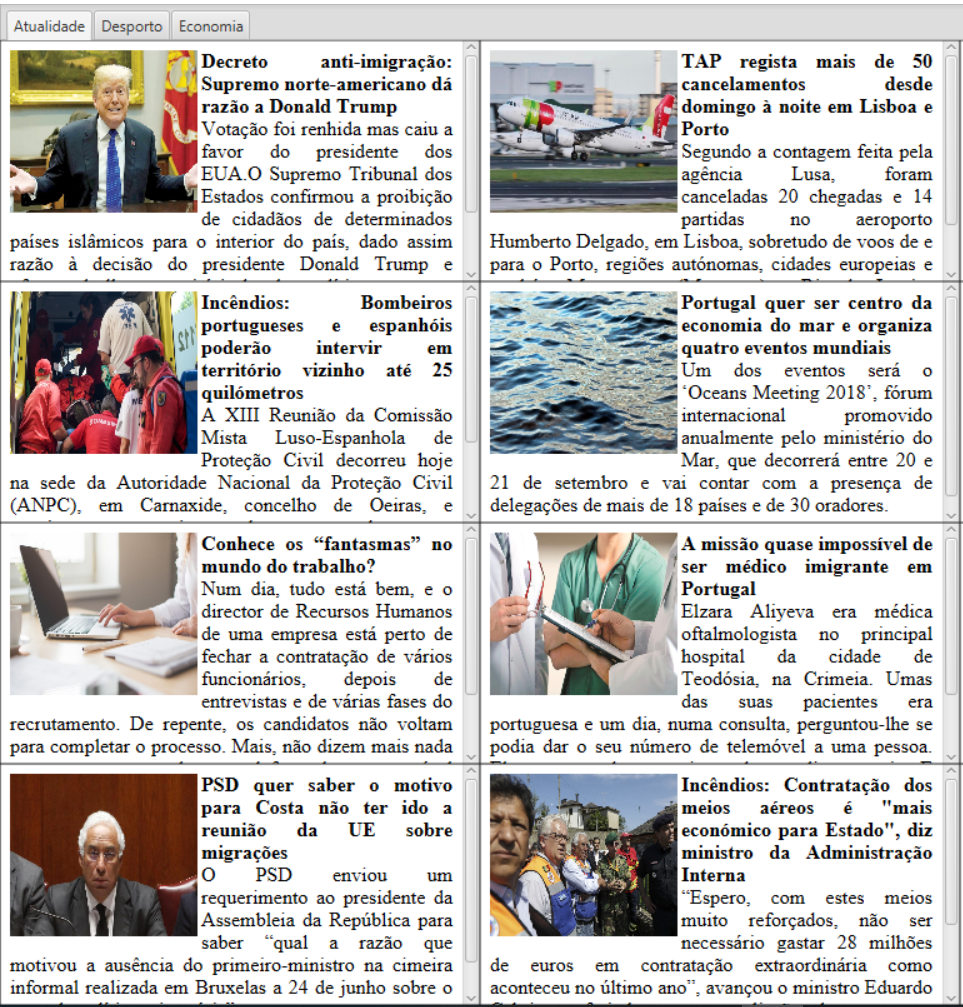
\includegraphics[scale=0.5]{imagens/app_img.png}
\caption{Imagem parcial da aplicação.}
\label{fig:gestao}
\end{figure}
A interface gráfica é particularmente simples de usar, tem como objetivo principal mostrar notícias e destacar aquelas que o utilizador considera mais importantes, através de um realçar da cor de fundo da própria notícia. Através do uso de separadores é possível escolher diferentes temas das notícias.\par
É possível atualizar as notícias carregando no botão \emph{"R"} e também são automaticamente atualizadas a cada meia hora, isto faz com que a aplicação esteja sempre atualizada.

\subsection{JSOUP}
\emph{Jsoup} é uma biblioteca \emph{Java} que permite analisar, manipular e extrair informações guardadas num documento \ac{HTML}. No âmbito deste projeto revelou-se muito importante, uma vez que através do \emph{Jsoup} que consegui manipular \emph{websites}, extraindo o seu código \ac{HTML} e a partir daí usar as informações a meu gosto.  \par 
Foram usadas várias funcionalidades do \emph{Jsoup}, tais como objetos do tipo \emph{Document},  que representam o código \ac{HTML} de uma página e objetos do tipo \emph{Element}, estes representam \emph{tags} \ac{HTML} e é a partir delas que navegamos pelo documento.

\begin{lstlisting}[language=Java, caption = Selecionar imagens de \emph{website} \label{code:imagens}]

try {
    Document document = Jsoup.connect(url).get();
    
    Elements locator = document.select("article[data-kpi] > figure > a > img");
            
    for (Element element : locator) {
        img_links.add(element.attr("src")); 
    }
    } catch (IOException e) {
        e.printStackTrace();
}
\end{lstlisting}
Na Listing 3.1 podemos observar em primeiro lugar que é feita uma conceção com o site, isto faz com que o código \ac{HTML} seja carregado para o objeto \emph{document}. \par
Pode-se observar o método \emph{select}, este permite encontrar elementos de acordo com uma \emph{query} feita ao documento.  O \emph{select} presente na imagem dá origem a todos as \emph{tags} \emph{img} que contêm a imagem de uma notícia. Considerando o código \ac{HTML} está estruturado como uma árvore, primeiro procura-se por uma \emph{tag} \emph{article} que contenha um atributo \emph{data-kpi}, a partir daqui procuram-se descendentes diretos (filhos), até encontrarmos a \emph{img} que pretendemos.
 A imagem seguinte revela exatamente o que foi descrito anteriormente.
\vspace{0,07cm}
\begin{figure}[H]
\centering
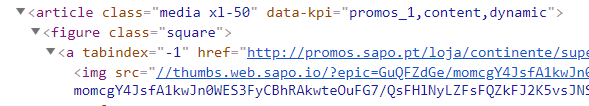
\includegraphics[scale=0.7]{imagens/html_img.PNG}
\caption{\emph{Tag img} com imagem da notícia.}
\label{fig:gestao}
\end{figure}



Este é um exemplo da utilização do \emph{Jsoup} no projeto, existem outros semelhantes que retiram o título das notícias ou o primeiro parágrafo da notícia, a técnica usado é em todo semelhante à do exemplo representado anteriormente.

\subsection{GitHub}
O \emph{GitHub} é um sistema de controlo de versões de código, através do qual  é possível realizar uma gestão mais eficaz do projeto sem correr o risco de apagar versões anteriores. Foi útil para este projeto porque permitiu guardar versões anteriores, muitas vezes ao implementar funcionalidades novas era possível testar versões anteriores em separado.
O repositório deste projecto pode ser consultado em \url{https://github.com/luisoliveira22/cristalNews.git}.


  

\section{Conclusões}
\label{chap3:sec:concs}
Neste capítulo foram descritas e caracterizadas detalhadamente as ferramentas e tecnologias usadas neste projeto, portanto, explicado o porquê da sua utilização.